\documentclass[tikz,border=2pt]{standalone}
\usepackage{amsmath,amssymb}
\usepackage{tikz}

\begin{document}
% Heine–Borel in R^2: a closed and bounded set (the closed disc) is compact — any open cover,
% here by small balls, can be thinned to finitely many that still cover it.
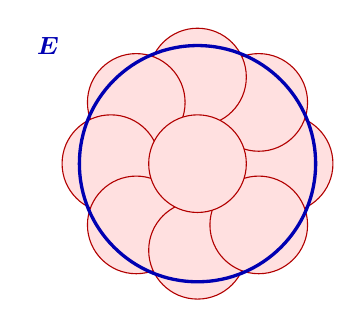
\begin{tikzpicture}[every node/.style={font=\small}]
	\fill[blue!15] (0,0) circle (1.5);
	\foreach \a in {0,45,...,315} {\draw[red!70!black, fill=red!12, fill opacity=1, draw opacity=1] ({1.1*cos(\a)},{1.1*sin(\a)}) circle (0.62);}
	\draw[red!70!black, fill=red!12] (0,0) circle (0.62);
	\draw[blue!70!black, very thick] (0,0) circle (1.5);
	\node[blue!70!black] at (-1.9,1.5) {$\boldsymbol{E}$};
\end{tikzpicture}
\end{document}
